\begin{frame}{Effective numeric performance}
    $$
    \mathcal{F} = \mathcal{C}_{\text{Cores}} * \mathcal{A}_{\text{AVX}} * \mathcal{V}_{\text{vector length}} * \mathcal{H}_{\text{Hyperthreading}} *\mathcal{F}_{\text{Freq}}
    $$
    Around 0.5 teraflops for a high-end laptop using stock overclock.
\end{frame}


\begin{frame}{Different parallel paradigms}
    \begin{figure}
        \centering
        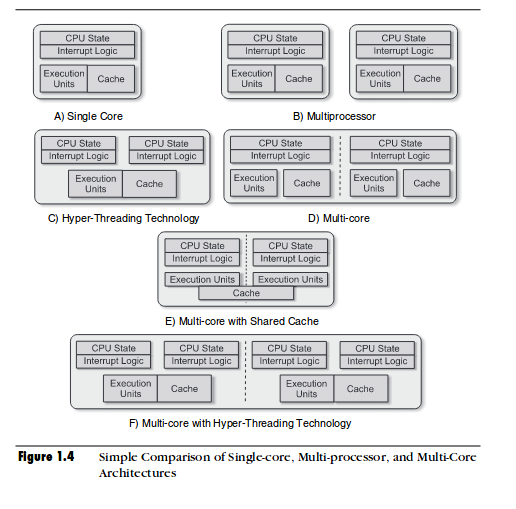
\includegraphics[width=0.8\textwidth]{png/hyperthread.png}
    \end{figure}
\end{frame}


\begin{frame}{Hyperthreading - Corporate version}
    Shut-up, it's magic ! \emph{Intel}
    \begin{figure}
        \centering
        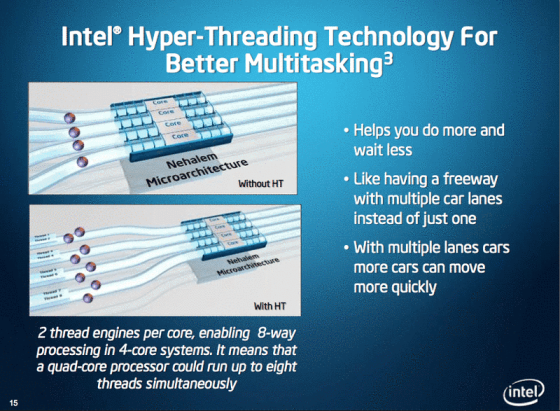
\includegraphics[width=0.8\textwidth]{png/intel_hyperthread.png}
    \end{figure}
\end{frame}

\begin{frame}{Hyperthreading - Honest version}
    Amazing (we cannot see the difference with real cores) for:
    \begin{itemize}
        \item Bad (for the meme) or heterogenous code
        \item Async, Async IO (Network operations, File access)
        \item Compiling your code
        \item Playing games (linked to first item)
        \item Battery, cost-per-unit
        \item Posting on messenger while your data gets Zucked
    \end{itemize}
    Ok (like sad 20\% improvement) for:
    \begin{itemize}
        \item Pure number crunching
    \end{itemize}
    Don't think there are downsides.
\end{frame}



\begin{frame}{Why should I care about SMP parallel programming ?}
    Embarrassingly parallel execution is king, unless
    \begin{itemize}
        \item Your task can be parallelized but is still heavily interlinked
        \item The algorithm is heavy and parallel (main sequence is long)
        \item You load a bunch of (common) data
        \item The main sequence is so small that process overhead is hard on you
    \end{itemize}
    \textbf{TL;DR:} You need \emph{Shared} memory.
\end{frame}
\begin{frame}{Different parallel paradigms}
    \begin{figure}
        \centering
        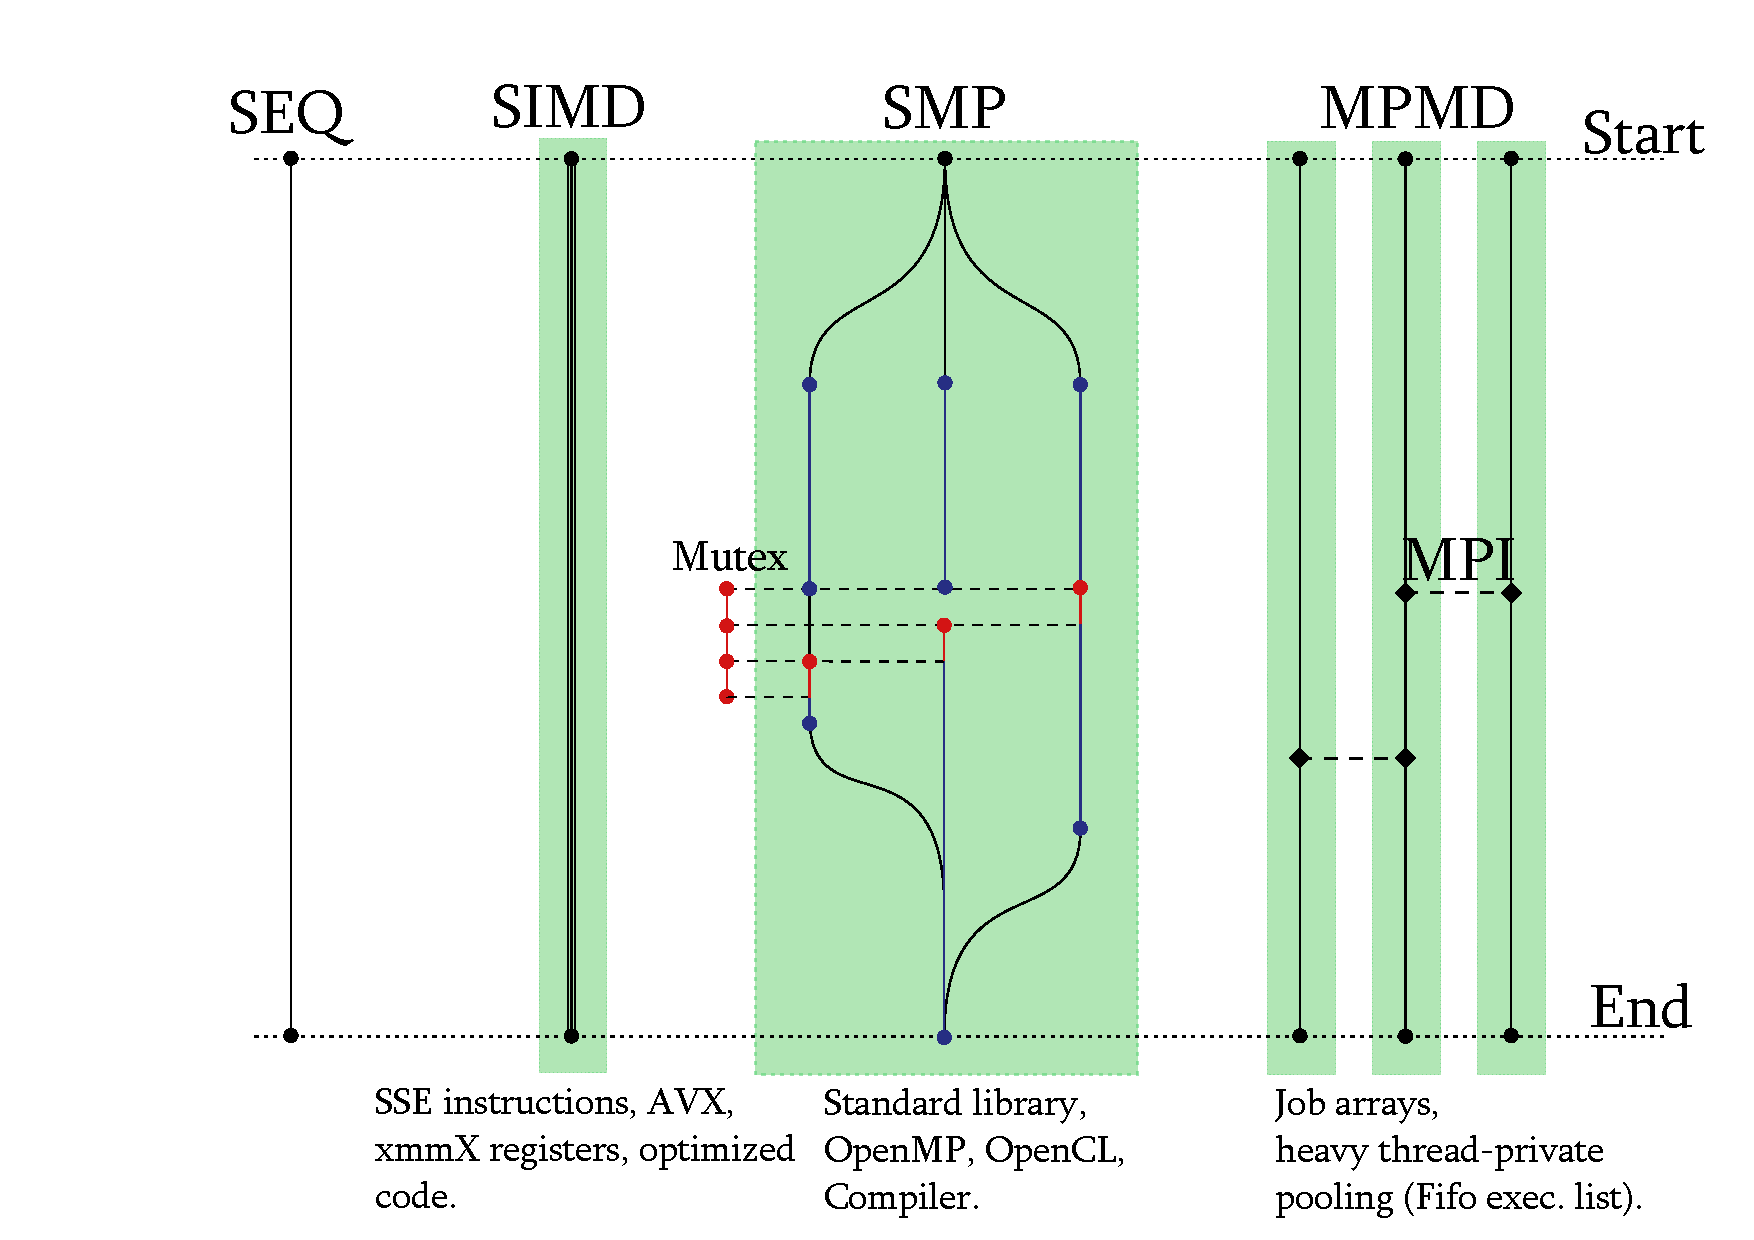
\includegraphics[width=1.0\textwidth]{pdf/parallelism.pdf}
    \end{figure}
\end{frame}
\begin{frame}{CPU architechture}
    \begin{figure}
        \centering
        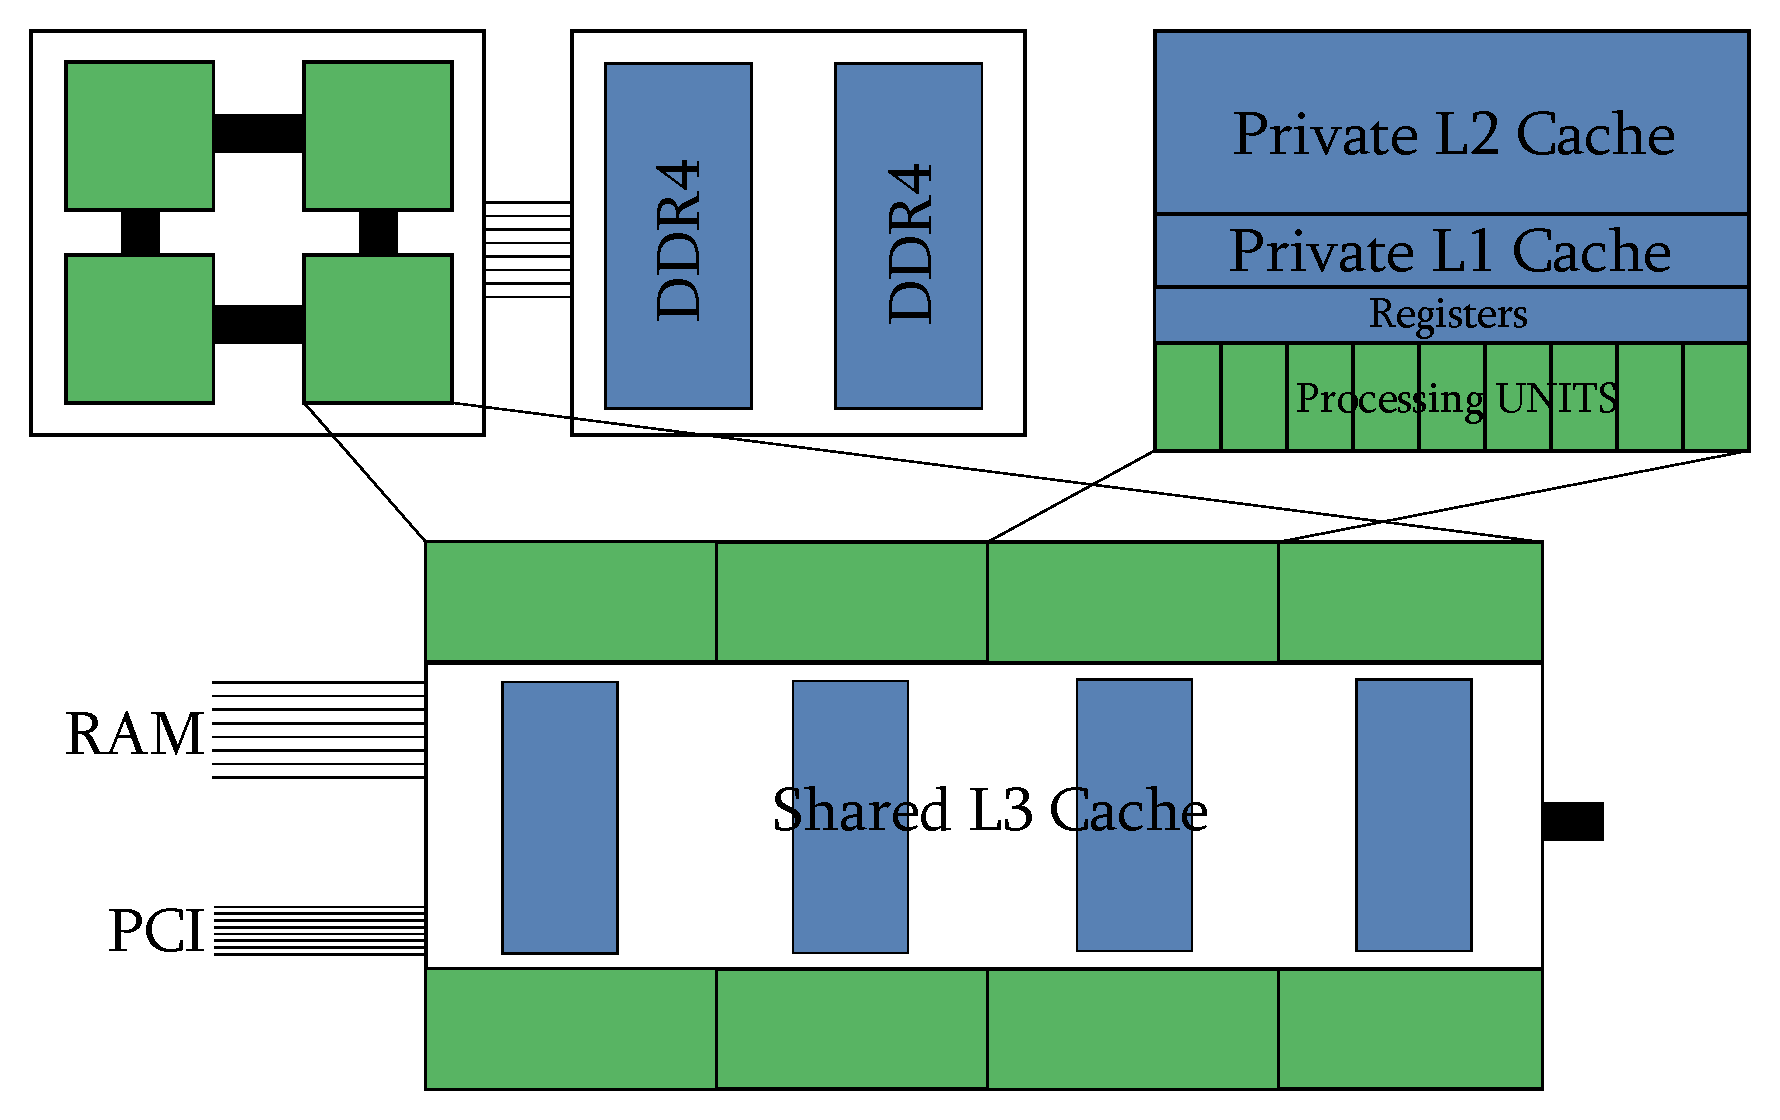
\includegraphics[width=1.0\textwidth]{pdf/architechture.pdf}
    \end{figure}
\end{frame}


\begin{frame}{Hyperthreading - Corporate version}
    Shut-up, it's magic ! \emph{Intel}
    \begin{figure}
        \centering
        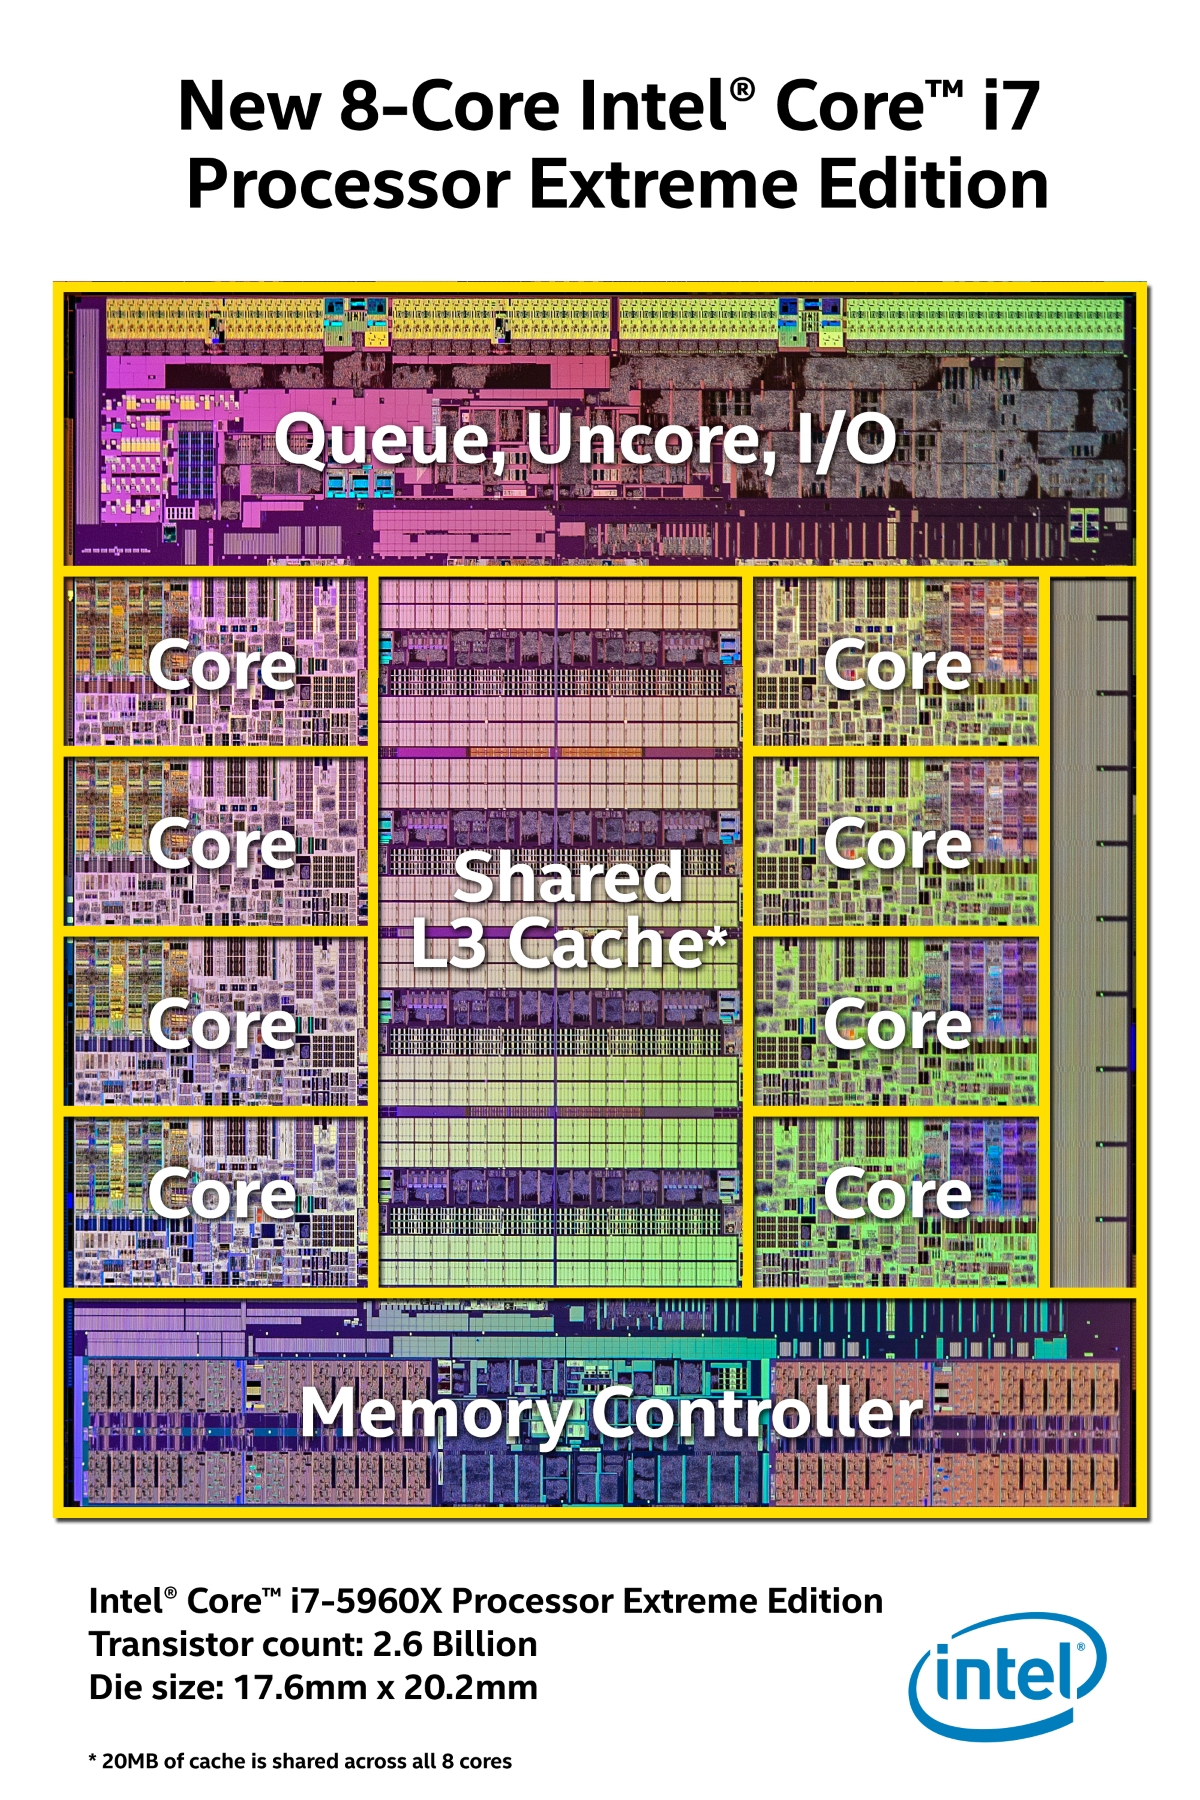
\includegraphics[width=0.8\textwidth]{png/die.png}
    \end{figure}
\end{frame}
\plain{Code: Manipulations de base (C++)}


